\subsubsection{Molecular Microbiology - Temperature Sensing}
\index{Ullrich, Matthias}


\paragraph{Research Team}

Matthias Ullrich (Professor), Annette Wensing (Postdoc), Helge Weingart (Postdoc), Yvonne Braun (PhD Student), Abhishek Srivastava (PhD Student), Daria Zhurina (PhD Student), Nehaya Al-Karablieh (PhD Student),
Poroshat Khalilpour (PhD Student), Astrid Gaerdes (Graduate Student)\\

A multiple approach is used to determine the influence of temperature on virulence and fitness enhancing gene expression in plant associated bacteria, such as Pseudomonas syringae and Erwinia amylovora. These phytopathogens cause devastating diseases on numerous host plants and represent excellent genetic model systems to investigate molecular plant-microbe interactions and pathogenicity. Our efforts focus on six major objectives: 1) the investigation of the regulation of biosynthesis of the phytotoxin coronatine; 2) the molecular analysis of cellular changes occurring at moderate temperature shifts; 3) the identification, analysis and molecular characterization of so far unknown thermo-responsive virulence and fitness determinants or secondary metabolites; 4) investigation of temperature-dependent protein secretion and exopolysaccharide synthesis; 5) molecular analysis of biofilm formation and silver toxicity; and 6) molecular and ecological investigations of multi-drug efflux pumps. Recently, a novel approach was launched to investigate the molecular interaction of marine heterotrophic bacteria with phytoplankton cells involved in carbon dioxide fixation in the ocean.

\paragraph{Highlights}
The year 2006 saw significant progress in a number of our research projects, from which the following three will be highlighted.

After the temperature-sensing mode of CorS, a histidine kinase involved in regulation of synthesis of the phytotoxin coronatine in Pseudomonas syringae, had been uncovered in the previous year, focus was set to generate hybrid kinases. These are composed of the N-terminal and C-terminal parts of CorS variants coming from temperature-dependent and temperature-independent strains of P. syringae. Our results suggested that both the N-terminal part of CorS as well as the presence of the cognate response regulator, CorR, from the temperature-dependent strain are important for full activity of CorS. Moreover, we identified another coronatine-producing strain which shows an opposite temperature behavior. With the help of this strain, we are going to further fine-analyze the temperature sensing mechanism of CorS.

The project on levansucrase, its regulation and secretion was intensified. The role of levan as nutritional storage compound in P. syringae biofilms could be demonstrated (Fig. \ref{fig:profUllrich}).
\begin{figure}[ht]
  \begin{center}
   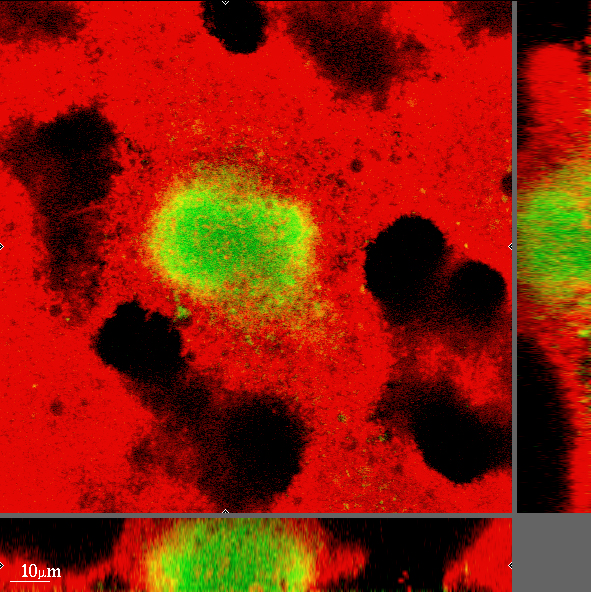
\includegraphics[width=\hsize]{Ullrich/profUllrich-fig1.png}
    \mycaption{ Binding of the lectin Concanavalin A (green) to levan accumulated in voids of biofilm microcolonies of \textit{Pseudomonas syringae} (red) using confocal laser scanning microscopy on flow chamber cultures of \textit{Pseudomonas syringae}. From Laue et al. (2006), Microbiology 152, 2909-2918. }\label{fig:profUllrich}
   \end{center}
\end{figure}

Levansucrase is an extracellular enzyme which occurs in two allelic
forms in P. syringae. It polymerizes fructosyl residues and thus
forms the exopolymer, levan. Interestingly and despite their close
similarity towards each other, both allelic enzymes occur in
different cellular compartments. Likewise, both genes, lscB and
lscC, are expressed in a clearly temperature-dependent manner. The
two PhD projects focusing on levansucrase have been directed towards
regulation and secretory mechanisms, respectively. The levansucrase
gene could be introduced into the levan-minus bacterium, Pseudomonas
putida, in order to identify regulators and/or the secretory pathway
for its gene product. Expression and secretion of levansucrase in P.
putida did not occur unless a genomic library of P. syringae was
provided. If so, three cosmids renders the P. putida transformants
levan-positive. After demonstrating that the levan formation of
these transformants was due to a simultaneous presence of cosmid and
lscB, the actual genes responsible for this phenotype were cloned
from the respective cosmids. Currently, we have zoomed into an
approximately 12-kb region containing several regulatory genes and
some hypothetical conserved genes. Regulation of levansucrase was
further studied by nested deletion analysis of the promoter region
of lscB. Approximately 440 bps upstream of the translational start
site are necessary to express lscB. Next steps will be to express
genes from the cosmids responsible for levansucrase expression in P.
putida, purify them and undertake DNA-protein interaction studies
with the minimal promoter sequence derived for lscB. Simultaneously,
a random mutagenesis was started to identify the transport system
for levansucrases.

A major highlight of this year's research was our participation at the research cruise ``VISION'' organized by the International Max Planck Research School for Marine Microbiology. Our research aimed at the analysis of interactions between heterotrophic marine bacteria with phytoplankton cells. This interaction is involved in the formation of marine snow which in turn contributes to carbon dioxide fixation in the ocean. This process is extremely relevant for global warming. Taking into account our previous results on plant-microbe interactions, the involvement of biofilm formation and exopolysaccharide synthesis, as well as multidrug efflux systems, our major aim is to identify a genetically feasible model organism which adheres to phytoplankton cells and is involved in aggregate formation. For this a marine transect was carried out obtaining more than 230 culturable bacterial isolates from water samples derived from 66�N,30�W to 30�N,30�W. Currently, the genetic feasibility of the isolates is analyzed. This novel project will allow us to study the interaction of a model strain with phytoplankton cultures and thus apply genetic tools to analyze this interaction at the molecular level.


\myparagraph{Collaborations}
Bremen Area Collaborations:
\begin{enumerate}
\item {\sl International University Bremen} \\ Prof. A. Boetius \\ Marine Microbiology
\\ Prof. F.O. Gl�ckner \\Expression profiling
 \\ Prof. A. Jeltsch  \\ Mass spectrometry
\\ Prof. V.B. Meyer-Rochow \\ Molecular taxonomy of mosses
 \\ Prof. G. Muskhelishvili \\ Promoter mapping
 \\ Prof. M. Winterhalter \\ Multidrug Efflux pumps
\item {\sl Alfred Wegner Institute for Polar Research} \\ Dr. U. Passow \\ Bacteria-phytoplankton interactions
\end{enumerate}
National \& International Collaborations:
\begin{enumerate}
\item {\sl BioCentrum Technical University of Denmark, Denmark} \\ Prof. S. Molin \\ Biofilm formation of Pseudomonas syringae
\item {\sl Friedrich Schiller University Jena} \\ Dr. B. Voelksch \\ Biocontrol of \textit{Pseudomonas syringae}
\item {\sl Oklahoma State University, Oklahoma, USA} \\ Prof. C.L. Bender \\ The alternative sigma factor AlgT
\item {\sl Michigan State University, Michigan, USA} \\ Prof. G.W. Sundin \\ Plasmid biology of \textit{Pseudomonas syringae}
\end{enumerate}


\paragraph{Grants}
\begin{enumerate}
\item Funded by DFG, \emph{Molecular analysis of the antagonistic
mechanisms within the interaction between \textit{Pseudomonas
syringae} strains inhabitating soybean leaf surfaces}, UL 169/2-3,
(May 2005  - December 2006)

\item Funded by DFG,  \emph{Dissection of the temperature-sensing
mechanism of the histidine protein kinase CorS from
  \textit{Pseudomonas syringae}}, UL 169/3-2, (November 2002 - December
  2006)
\item Funded by DFG, \emph{Genome-wide analysis of multidrug
efflux in the plant-pathogenic bacterium \textit{Pseudomonas
syringae}}, UL 169/4-1, (November 2005 - October 2007)
\end{enumerate}

\paragraph{Other Support Grants}
\begin{enumerate}
\item EU ``Marie Curie Early Training Stage, Molecular analysis of the thermo-responsive secretion mechanism for two alleles of levansucrase in \textit{Pseudomonas syringae}''
\item  DAAD ``Identification of plant-borne inhibitors of multidrug efflux-mediated resistance in the fire blight pathogen, \textit{Erwinia amylovora}''
\item BioGate AG ``Molecular analysis of the influence of nano-structured silver in polymer surfaces on biofilm-producing microorganisms''
\end{enumerate}

\nocite{Ullrich1,Ullrich2,Ullrich3,Ullrich4,Ullrich5,Ullrich6,Ullrich7}
